\documentclass[10pt,aspectratio=169]{beamer}

% ============================================================
% Módulo 3: Construcción de Escenarios Macro-Financieros
% Curso: Stress Testing en Sistemas de Pensiones de Capitalización Individual
% MACROPOL
% Versión reorganizada para mayor coherencia narrativa
% ============================================================

\usetheme{metropolis}
\usecolortheme{seahorse}
\usefonttheme{professionalfonts}

\usepackage[spanish,es-noquoting]{babel}
\usepackage[utf8]{inputenc}
\usepackage[T1]{fontenc}
\usepackage{amsmath,amssymb,bm}
\usepackage{booktabs}
\usepackage{array}
\usepackage{graphicx}
\usepackage{tikz}
\usepackage{listings}
\usepackage{xcolor}
\usepackage{courier}
\usepackage{graphicx}
\usetikzlibrary{arrows.meta,positioning,calc}

\renewcommand{\ttdefault}{pcr}
% ------------------------------------------------------------
% Colores
% ------------------------------------------------------------
\definecolor{MacropolBlue}{RGB}{0,67,122}
\definecolor{MacropolTeal}{RGB}{0,134,150}
\definecolor{MacropolGray}{RGB}{80,80,80}
\definecolor{SoftBlue}{RGB}{235,244,250}
\definecolor{SoftRed}{RGB}{252,238,238}
\definecolor{SoftGreen}{RGB}{235,248,240}
\definecolor{CodeBg}{RGB}{248,248,248}

\setbeamercolor{title}{fg=MacropolBlue}
\setbeamercolor{frametitle}{fg=MacropolBlue}
\setbeamercolor{structure}{fg=MacropolBlue}
\setbeamercolor{block title}{bg=MacropolBlue,fg=white}
\setbeamercolor{block body}{bg=SoftBlue,fg=black}
\setbeamertemplate{navigation symbols}{}
\setbeamertemplate{footline}[frame number]

% ------------------------------------------------------------
% R listings
% ------------------------------------------------------------
\lstdefinelanguage{R}{
  keywords={function,if,else,for,while,repeat,in,next,break,TRUE,FALSE,NULL,NA,NaN,Inf},
  otherkeywords={<-,<<-,$,~},
  sensitive=true,
  morecomment=[l]\#,
  morestring=[b]",
  morestring=[b]'
}

\lstset{
  language=R,
  basicstyle=\ttfamily\scriptsize,
  keywordstyle=\color{MacropolBlue}\bfseries,
  commentstyle=\color{MacropolGray}\itshape,
  stringstyle=\color{MacropolTeal},
  backgroundcolor=\color{CodeBg},
  frame=single,
  rulecolor=\color{MacropolGray!40},
  breaklines=true,
  showstringspaces=false,
  columns=fullflexible
}

% ------------------------------------------------------------
% Macros
% ------------------------------------------------------------
\newcommand{\baseline}{\textcolor{MacropolTeal}{\textbf{baseline}}}
\newcommand{\adverso}{\textcolor{red!70!black}{\textbf{adverso}}}
\newcommand{\R}{\texttt{R}}
\newcommand{\dd}{\mathrm{d}}

% ------------------------------------------------------------
% Metadata
% ------------------------------------------------------------
\title[Stress Testing Pensiones -- Módulo 3]{Módulo 3: Construcción de Escenarios Macro-Financieros}
\subtitle{ARIMA, VAR, Monte Carlo y diseño de choques para sistemas de pensiones}
\author{MACROPOL: Economía Aplicada y Políticas Públicas}
\institute{Curso: Stress Testing en Sistemas de Pensiones de Capitalización Individual}
\date{}

\begin{document}

% ============================================================
% PARTE I: INTRODUCCIÓN
% ============================================================

\begin{frame}
\titlepage
\end{frame}

% ============================================================
\begin{frame}{¿Dónde estamos en el curso?}
\begin{block}{Módulo 3 dentro del flujo de stress testing previsional}
El módulo transforma una \textbf{narrativa macroeconómica} en trayectorias cuantitativas de variables que luego alimentan el stress test del portafolio, el módulo actuarial y el reporte regulatorio.
\end{block}

\begin{center}
\begin{tikzpicture}[node distance=0.5cm, every node/.style={font=\scriptsize}]
\node[draw, rounded corners, fill=SoftBlue, minimum width=2.4cm, minimum height=0.8cm] (m1) {M1 Fundamentos};
\node[draw, rounded corners, fill=SoftBlue, right=of m1, minimum width=2.6cm, minimum height=0.8cm] (m2) {M2 Riesgos};
\node[draw, rounded corners, fill=SoftGreen, right=of m2, minimum width=3.0cm, minimum height=0.8cm] (m3) {\textbf{M3 Escenarios}};
\node[draw, rounded corners, fill=SoftBlue, right=of m3, minimum width=2.7cm, minimum height=0.8cm] (m4) {M4 Portafolio};
\node[draw, rounded corners, fill=SoftBlue, below=0.7cm of m4, minimum width=2.7cm, minimum height=0.8cm] (m5) {M5 Actuarial};
\node[draw, rounded corners, fill=SoftBlue, left=of m5, minimum width=3.0cm, minimum height=0.8cm] (m6) {M6 Reporte};

\draw[-{Latex}, thick] (m1) -- (m2);
\draw[-{Latex}, thick] (m2) -- (m3);
\draw[-{Latex}, thick] (m3) -- (m4);
\draw[-{Latex}, thick] (m4) -- (m5);
\draw[-{Latex}, thick] (m5) -- (m6);
\end{tikzpicture}
\end{center}

\textbf{Producto del módulo:} matriz de escenarios macro-financieros por horizonte, variable y severidad.
\end{frame}

% ============================================================
\begin{frame}{Objetivos de aprendizaje}
Al finalizar el módulo, los participantes podrán:

\begin{enumerate}
  \item Construir un escenario \baseline{} y uno \adverso{} para variables macro-financieras relevantes.
  \item Estimar modelos ARIMA para proyecciones univariadas.
  \item Estimar modelos VAR para capturar interdependencias macro-financieras.
  \item Generar trayectorias Monte Carlo y bandas de incertidumbre.
  \item Calibrar choques históricos e hipotéticos con trazabilidad regulatoria.
  \item Implementar un flujo reproducible en \R{}.
\end{enumerate}

\vspace{0.4em}
\begin{block}{Principio conductor}
No buscamos ``predecir el futuro''. Buscamos construir trayectorias \textbf{coherentes, severas y plausibles} para evaluar la resiliencia del sistema previsional.
\end{block}
\end{frame}

% ============================================================
\begin{frame}{Ruta gradual del módulo}
\begin{center}
\begin{tikzpicture}[node distance=0.35cm, every node/.style={font=\scriptsize}]
\node[draw, rounded corners, fill=SoftBlue, minimum width=2.5cm, minimum height=0.8cm] (n1) {1. Contexto};
\node[draw, rounded corners, fill=SoftBlue, right=of n1, minimum width=2.5cm, minimum height=0.8cm] (n2) {2. Datos};
\node[draw, rounded corners, fill=SoftBlue, right=of n2, minimum width=2.5cm, minimum height=0.8cm] (n3) {3. ARIMA};
\node[draw, rounded corners, fill=SoftBlue, right=of n3, minimum width=2.5cm, minimum height=0.8cm] (n4) {4. VAR};
\node[draw, rounded corners, fill=SoftBlue, below=0.55cm of n4, minimum width=2.5cm, minimum height=0.8cm] (n5) {5. Monte Carlo};
\node[draw, rounded corners, fill=SoftBlue, left=of n5, minimum width=2.5cm, minimum height=0.8cm] (n6) {6. Choques};
\node[draw, rounded corners, fill=SoftGreen, left=of n6, minimum width=2.5cm, minimum height=0.8cm] (n7) {7. Taller R};

\draw[-{Latex}, thick] (n1) -- (n2);
\draw[-{Latex}, thick] (n2) -- (n3);
\draw[-{Latex}, thick] (n3) -- (n4);
\draw[-{Latex}, thick] (n4) -- (n5);
\draw[-{Latex}, thick] (n5) -- (n6);
\draw[-{Latex}, thick] (n6) -- (n7);
\end{tikzpicture}
\end{center}

\begin{columns}
\column{0.48\textwidth}
\begin{block}{De menor a mayor complejidad}
\begin{itemize}
  \item Una variable: ARIMA.
  \item Varias variables: VAR.
  \item Muchas trayectorias: Monte Carlo.
  \item Narrativa adversa: choques calibrados.
\end{itemize}
\end{block}
\column{0.48\textwidth}
\begin{block}{De modelo a decisión}
\begin{itemize}
  \item Escenarios reproducibles.
  \item Supuestos auditables.
  \item Impactos comparables.
  \item Reglas de acción supervisora.
\end{itemize}
\end{block}
\end{columns}
\end{frame}

% ============================================================
\section{1. De los shocks macro a las pensiones}

% ============================================================
\begin{frame}{¿Qué es un escenario macro-financiero?}
\begin{block}{Definición operativa}
Un escenario es una trayectoria conjunta de variables macroeconómicas y financieras bajo una narrativa específica, con horizonte, frecuencia, severidad y supuestos explícitos.
\end{block}

\begin{table}
\small
\begin{tabular}{p{3.2cm}p{4.2cm}p{4.2cm}}
\toprule
Componente & \baseline{} & \adverso{} \\
\midrule
Narrativa & Normalización gradual & Desaceleración + tasas altas + depreciación \\
Modelo & Proyección central & Proyección condicionada a choques \\
Supuestos & Política y mercado sin disrupciones & Persistencia de inflación y prima de riesgo \\
Resultado & Trayectoria esperada & Pérdida de valor y deterioro de aportes \\
\bottomrule
\end{tabular}
\end{table}
\end{frame}

% ============================================================
\begin{frame}{De shocks macroeconómicos a resultados previsionales}
\begin{center}
\begin{tikzpicture}[node distance=0.62cm, every node/.style={font=\scriptsize}]
\node[draw, rounded corners, fill=SoftRed, minimum width=2.8cm, minimum height=0.8cm] (shock) {Shock macro};
\node[draw, rounded corners, fill=SoftBlue, right=of shock, minimum width=3.0cm, minimum height=0.8cm] (channels) {Canales};
\node[draw, rounded corners, fill=SoftBlue, right=of channels, minimum width=3.0cm, minimum height=0.8cm] (risk) {Factores de riesgo};
\node[draw, rounded corners, fill=SoftGreen, right=of risk, minimum width=3.0cm, minimum height=0.8cm] (result) {Resultados previsionales};

\draw[-{Latex}, thick] (shock) -- (channels);
\draw[-{Latex}, thick] (channels) -- (risk);
\draw[-{Latex}, thick] (risk) -- (result);
\end{tikzpicture}
\end{center}

\vspace{0.35cm}

\begin{columns}[T]
\column{0.48\textwidth}
\begin{block}{Canal financiero}
\begin{itemize}
  \item Tasa de interés local.
  \item Inflación y tasa real.
  \item Tipo de cambio.
  \item Spread soberano.
  \item Rentabilidad de bonos y renta variable.
\end{itemize}
\end{block}

\column{0.48\textwidth}
\begin{block}{Canal previsional}
\begin{itemize}
  \item Salario real.
  \item Empleo formal.
  \item Densidad de cotización.
  \item Aportes.
  \item Saldo acumulado.
\end{itemize}
\end{block}
\end{columns}

\vspace{0.25cm}
\begin{block}{Transición conceptual}
Las variables de estos canales funcionan como \textbf{factores de transmisión del riesgo} hacia el sistema previsional.
\end{block}
\end{frame}

% ============================================================
\begin{frame}{¿Qué son los factores de riesgo?}
En un sistema de capitalización individual, los \textbf{factores de riesgo} son variables que afectan:

\begin{itemize}
    \item el valor del portafolio previsional;
    \item el saldo acumulado del afiliado;
    \item la pensión esperada;
    \item la tasa de reemplazo.
\end{itemize}

\begin{block}{Definición}
Un factor de riesgo es toda variable que, al cambiar, modifica los activos, pasivos o beneficios previsionales.
\end{block}

\vspace{0.2cm}
\textbf{Idea clave:} no se estresa directamente la pensión; se estresan los factores que la determinan.
\end{frame}

% ============================================================
\begin{frame}{Tipos de factores de riesgo previsional}
\begin{columns}[T]

\begin{column}{0.32\textwidth}
\begin{block}{Macroeconómicos}
\begin{itemize}
    \item PIB.
    \item Inflación.
    \item Tasas de interés.
    \item Desempleo.
\end{itemize}
\end{block}
\end{column}

\begin{column}{0.32\textwidth}
\begin{block}{Financieros}
\begin{itemize}
    \item Retornos.
    \item Volatilidad.
    \item Correlaciones.
    \item Riesgo de crédito.
\end{itemize}
\end{block}
\end{column}

\begin{column}{0.32\textwidth}
\begin{block}{Actuariales}
\begin{itemize}
    \item Longevidad.
    \item Edad de retiro.
    \item Densidad de cotización.
    \item Trayectoria salarial.
\end{itemize}
\end{block}
\end{column}

\end{columns}

\vspace{0.45cm}
\begin{exampleblock}{Ejemplo de portafolio}
\[
R_p = \sum_{i=1}^{N} w_i R_i
\]
Los factores de riesgo incluyen retornos, volatilidades y correlaciones:
\[
R_i,\quad \sigma_i,\quad \rho_{ij}
\]
\end{exampleblock}
\end{frame}

% ============================================================
\begin{frame}{Baseline vs. escenario adverso}
\textbf{Del factor de riesgo al impacto previsional}

\vspace{0.2cm}

\begin{table}
\centering
\small
\begin{tabular}{lcc}
\hline
\textbf{Factor} & \textbf{Baseline} & \textbf{Escenario adverso} \\
\hline
Retornos financieros & normales & caída de mercado \\
Tasa de interés & estable & shock de tasas \\
Inflación & controlada & aumento persistente \\
Longevidad & tendencia esperada & mayor esperanza de vida \\
Densidad de cotización & estable & caída por desempleo \\
\hline
\end{tabular}
\end{table}

\vspace{0.3cm}

\begin{block}{Intuición económica}
\begin{itemize}
    \item Shock financiero $\rightarrow$ menor saldo acumulado.
    \item Shock de longevidad $\rightarrow$ menor pensión mensual.
    \item Shock laboral $\rightarrow$ menor densidad de cotización.
    \item Shock combinado $\rightarrow$ deterioro de la tasa de reemplazo.
\end{itemize}
\end{block}

\textbf{Lectura regulatoria:} identificar qué factores explican la vulnerabilidad permite diseñar respuestas de política pública.
\end{frame}

% ============================================================
\begin{frame}{Modelo conceptual del escenario}
\begin{center}
\begin{tikzpicture}[node distance=0.6cm, every node/.style={font=\scriptsize}]
\node[draw, rounded corners, fill=SoftBlue, minimum width=3.0cm, minimum height=0.9cm] (data) {Datos históricos};
\node[draw, rounded corners, fill=SoftBlue, right=of data, minimum width=3.0cm, minimum height=0.9cm] (model) {Modelo estadístico};
\node[draw, rounded corners, fill=SoftRed, right=of model, minimum width=3.0cm, minimum height=0.9cm] (shock) {Choque adverso};
\node[draw, rounded corners, fill=SoftGreen, below=0.8cm of model, minimum width=3.6cm, minimum height=0.9cm] (scenario) {Trayectoria del escenario};
\node[draw, rounded corners, fill=SoftBlue, right=of scenario, minimum width=3.1cm, minimum height=0.9cm] (use) {Inputs M4--M5};

\draw[-{Latex}, thick] (data) -- (model);
\draw[-{Latex}, thick] (model) -- (shock);
\draw[-{Latex}, thick] (model) -- (scenario);
\draw[-{Latex}, thick] (shock) -- (scenario);
\draw[-{Latex}, thick] (scenario) -- (use);
\end{tikzpicture}
\end{center}

\begin{block}{Separación clave}
\textbf{Narrativa económica}: por qué ocurre el shock. \\
\textbf{Modelo cuantitativo}: cómo se propaga a las variables. \\
\textbf{Resultado}: cuánto cambia el balance previsional.
\end{block}
\end{frame}

% ============================================================
\section{2. Datos y preparación del taller}

% ============================================================
\begin{frame}{Datos: estructura mínima para el taller}
\begin{table}
\small
\begin{tabular}{lll}
\toprule
Variable & Frecuencia sugerida & Transformación \\
\midrule
PIB real / IMAE & Mensual/Trimestral & Crecimiento interanual o trimestral anualizado \\
Inflación & Mensual / trimestral & Variación anual o trimestral \\
Tasa de política & Mensual / trimestral & Nivel o cambio en puntos básicos \\
Tipo de cambio & Mensual / trimestral & Depreciación porcentual \\
Spread soberano & Mensual / trimestral & Nivel o cambio en puntos básicos \\
Rentabilidad fondo & Mensual / trimestral & Retorno logarítmico \\
Salario real & Mensual / trimestral & Crecimiento real \\
\bottomrule
\end{tabular}
\end{table}

\begin{block}{Regla práctica}
El modelo más sofisticado no compensa datos mal transformados. La consistencia de frecuencia, unidades y signos es parte del control regulatorio.
\end{block}
\end{frame}

% ============================================================
\begin{frame}[fragile]{Implementación: plantilla de datos en R}
\begin{lstlisting}
# Paquetes sugeridos
library(readr)
library(dplyr)
library(lubridate)
library(tsibble)

datos <- read_csv("datos_macro_pensiones.csv") %>%
  mutate(fecha = ymd(fecha)) %>%
  arrange(fecha)

# Variables transformadas
datos_modelo <- datos %>%
  mutate(
    inflacion = 100 * (log(ipc) - lag(log(ipc), 12)),
    deprec_fx = 100 * (log(tc) - lag(log(tc), 12)),
    ret_fondo = 100 * (log(valor_cuota) - lag(log(valor_cuota))),
    salario_real = 100 * (log(salario_nominal/ipc) -
                          lag(log(salario_nominal/ipc), 12))
  ) %>%
  tidyr::drop_na()
\end{lstlisting}
\end{frame}

% ============================================================
\section{3. De shocks a trayectorias cuantitativas}

% ============================================================
\begin{frame}{Problema central del stress testing}
Los escenarios macroeconómicos no impactan directamente las pensiones. El desafío técnico es convertir una narrativa de estrés en trayectorias cuantificables de factores de riesgo.

\vspace{0.3cm}

\begin{block}{Pregunta operativa}
¿Cómo transformar un \textbf{shock macro} en cambios cuantificables en retornos, tasas, salarios, empleo y densidad de cotización?
\end{block}

\vspace{0.25cm}

\begin{center}
\begin{tikzpicture}[node distance=0.65cm, every node/.style={font=\scriptsize}]
\node[draw, rounded corners, fill=SoftRed, minimum width=2.8cm, minimum height=0.8cm] (shock) {Shock macro};
\node[draw, rounded corners, fill=SoftBlue, right=of shock, minimum width=3.0cm, minimum height=0.8cm] (macro) {Variables macro};
\node[draw, rounded corners, fill=SoftBlue, right=of macro, minimum width=3.0cm, minimum height=0.8cm] (risk) {Factores de riesgo};
\node[draw, rounded corners, fill=SoftGreen, right=of risk, minimum width=2.8cm, minimum height=0.8cm] (pension) {Pensión};
\draw[-{Latex}, thick] (shock) -- (macro);
\draw[-{Latex}, thick] (macro) -- (risk);
\draw[-{Latex}, thick] (risk) -- (pension);
\end{tikzpicture}
\end{center}
\end{frame}

% ============================================================
\begin{frame}{¿Por qué usar modelos de series de tiempo?}
\begin{table}
\small
\begin{tabular}{p{3.0cm}p{4.4cm}p{4.2cm}}
\toprule
Herramienta & Función & Uso previsional \\
\midrule
ARIMA & Dinámica individual de una variable & Baseline de inflación, tasas, salarios o retornos \\
VAR & Interacción entre variables & Propagación de shocks macro-financieros \\
Monte Carlo & Muchas trayectorias posibles & Distribución de pérdidas, umbrales y percentiles \\
Choques calibrados & Severidad histórica o hipotética & Escenarios adversos defendibles \\
\bottomrule
\end{tabular}
\end{table}

\begin{exampleblock}{Mensaje clave}
ARIMA, VAR y Monte Carlo permiten traducir narrativas macro en \textbf{trayectorias cuantitativas coherentes} para el stress testing.
\end{exampleblock}
\end{frame}

% ============================================================
\begin{frame}{Intuición económica de transmisión}
\begin{block}{Canales típicos}
\begin{itemize}
    \item Recesión $\rightarrow$ menor PIB $\rightarrow$ menor empleo $\rightarrow$ menor densidad de cotización.
    \item Crisis financiera $\rightarrow$ menores retornos $\rightarrow$ menor saldo acumulado.
    \item Inflación persistente $\rightarrow$ menor tasa real $\rightarrow$ menor rendimiento real.
    \item Depreciación cambiaria $\rightarrow$ mayor inflación $\rightarrow$ respuesta de tasas $\rightarrow$ pérdida en bonos.
\end{itemize}
\end{block}

\vspace{0.3cm}
\textbf{Transición:} primero construimos una trayectoria central por variable; luego introducimos interdependencias y choques conjuntos.
\end{frame}

% ============================================================
\section{4. Modelos ARIMA}

% ============================================================
\begin{frame}{Contexto: ¿cuándo usar ARIMA en escenarios previsionales?}
\begin{block}{Uso principal}
ARIMA es el punto de entrada para construir trayectorias \baseline{} de una variable individual cuando queremos capturar persistencia, reversión y shocks idiosincráticos.
\end{block}

\begin{columns}
\column{0.48\textwidth}
\begin{block}{Útil para}
\begin{itemize}
  \item Inflación.
  \item Tasa de interés.
  \item Rentabilidad agregada.
  \item Salario real.
\end{itemize}
\end{block}

\column{0.48\textwidth}
\begin{block}{Limitación}
\begin{itemize}
  \item No impone coherencia entre variables.
  \item No explica contagio macro-financiero.
  \item Es más débil para escenarios condicionados.
\end{itemize}
\end{block}
\end{columns}
\end{frame}

% ============================================================
\begin{frame}{Modelo / Herramienta: ARIMA}
Sea $y_t$ una variable macro-financiera. Un modelo ARIMA$(p,d,q)$ se define como:

\[
\phi(L)(1-L)^d y_t = c + \theta(L)\varepsilon_t,
\quad \varepsilon_t \sim (0,\sigma^2)
\]

\begin{itemize}
  \item $p$: rezagos autorregresivos.
  \item $d$: diferenciación necesaria para estacionariedad.
  \item $q$: rezagos del error.
  \item $\phi(L)$ y $\theta(L)$: polinomios en el operador rezago.
\end{itemize}

\begin{block}{Intuición económica}
El pasado reciente contiene información sobre la velocidad de reversión, persistencia inflacionaria o inercia de tasas. ARIMA formaliza esa memoria.
\end{block}
\end{frame}

% ============================================================
\begin{frame}{ARIMA: flujo de estimación gradual}
\begin{enumerate}
  \item Graficar la serie y detectar quiebres, tendencia o estacionalidad.
  \item Transformar: log, diferencias, tasas de crecimiento.
  \item Evaluar estacionariedad.
  \item Seleccionar $(p,d,q)$ por AIC/BIC y criterio económico.
  \item Diagnosticar residuos.
  \item Proyectar \baseline{}.
  \item Condicionar o desplazar la trayectoria para un \adverso{} simple.
\end{enumerate}

\vspace{0.4em}
\begin{block}{Regla de enseñanza}
Primero se valida la historia económica de la serie; luego se valida la especificación estadística.
\end{block}
\end{frame}

% ============================================================
\begin{frame}[fragile]{Implementación: ARIMA para inflación (\texttt{arima\_inflacion.R})}
\begin{lstlisting}
library(forecast)
library(ggplot2)

# Serie mensual de inflacion
infl_ts <- ts(datos_modelo$inflacion,
              start = c(2007, 1), frequency = 12)

# Seleccion automatica, pero revisada por el analista
fit_arima <- auto.arima(infl_ts,
                        seasonal = FALSE,
                        stepwise = FALSE,
                        approximation = FALSE)

summary(fit_arima)
checkresiduals(fit_arima)

# Proyeccion baseline
fc_base <- forecast(fit_arima, h = 8, level = c(50, 80, 95))
autoplot(fc_base)
\end{lstlisting}
\end{frame}

% ============================================================
\begin{frame}{De ARIMA a escenario adverso de inflación}
\footnotesize
\begin{block}{Regla general}
\[
\pi^{adv}_{t+h} = \hat{\pi}_{t+h} + k_h \cdot \sigma_{\varepsilon}
\]
\end{block}

\begin{itemize}
\item $\hat{\pi}_{t+h}$: pronóstico baseline ARIMA.
\item $\sigma_{\varepsilon}$: desviación estándar de residuos.
\item $k_h$: perfil dinámico del shock.
\end{itemize}

\vspace{0.35cm}

\begin{block}{Perfil del shock ($k_h$)}
\begin{center}
\begin{tabular}{lcc}
\toprule
Horizonte & $k_h$ & Interpretación \\
\midrule
$t+1$ & 1.5 & shock máximo \\
$t+2$ & 1.5 & persistencia \\
$t+3$ & 1.5 & persistencia \\
$t+4$ & 1.0 & inicio reversión \\
$t+5$ & 0.8 & reversión \\
$t+6$ & 0.5 & disipación \\
$t+7+$ & 0.0 & normalización \\
\bottomrule
\end{tabular}
\end{center}
\end{block}
\end{frame}

% ============================================================
\begin{frame}{De ARIMA a escenario adverso de inflación}
\begin{block}{Traducción a puntos porcentuales}
\[
Shock_{t+h} = k_h \cdot \sigma_{\varepsilon}
\]
\small
Ejemplo: si $\sigma = 0.8$, entonces shock máximo $= 1.5 \times 0.8 = 1.2$ p.p.
\end{block}

\vspace{0.3cm}

\begin{alertblock}{Supuesto clave}
La tasa nominal se mantiene constante para aislar el efecto inflacionario.
\end{alertblock}
\end{frame}

% ============================================================
\begin{frame}{Supuestos vs resultados del escenario}
\begin{columns}

\column{0.48\textwidth}
\begin{block}{Supuestos}
\begin{itemize}
\item Horizonte: 24 meses.
\item Shock máximo: $1.5\sigma$.
\item Persistencia: 3 meses.
\item Reversión: gradual.
\item Tasa nominal: baseline.
\end{itemize}
\end{block}

\column{0.48\textwidth}
\begin{block}{Resultados}
\begin{itemize}
\item Inflación máxima.
\item Shock en puntos porcentuales.
\item Tasa real mínima.
\item Meses con tasa real negativa.
\end{itemize}
\end{block}

\end{columns}

\vspace{0.4cm}

\begin{alertblock}{Mensaje clave}
El modelo ARIMA genera el baseline. El escenario adverso depende de supuestos explícitos del analista.
\end{alertblock}
\end{frame}

% ============================================================
\begin{frame}{Ejercicio ARIMA (\texttt{ejercicio\_ARIMA\_simple.R})}
\begin{block}{Caso aplicado}
El regulador requiere un escenario de inflación para evaluar el retorno real de los fondos de pensiones durante los próximos 8 trimestres.
\end{block}

\begin{enumerate}
  \item Estimar un ARIMA para inflación.
  \item Generar la trayectoria \baseline{}.
  \item Construir un \adverso{} con inflación 1.5 desviaciones estándar por encima del baseline durante cuatro trimestres.
  \item Calcular tasa real aproximada:
  \[
  r^{real}_t \approx i_t - \pi_t
  \]
\end{enumerate}
\end{frame}

% ============================================================
\begin{frame}{Interpretación ARIMA para decisión regulatoria}
\begin{columns}
\column{0.48\textwidth}
\begin{block}{Qué mirar}
\begin{itemize}
  \item Persistencia del shock.
  \item Ancho de intervalos de predicción.
  \item Sesgo de residuos.
  \item Sensibilidad del retorno real.
\end{itemize}
\end{block}

\column{0.48\textwidth}
\begin{block}{Decisiones posibles}
\begin{itemize}
  \item Exigir escenarios de inflación más severos.
  \item Revisar supuestos de tasa real.
  \item Pedir análisis de sensibilidad de portafolio.
  \item Alinear horizonte con madurez de activos.
\end{itemize}
\end{block}
\end{columns}

\vspace{0.4em}
\begin{block}{Mensaje}
ARIMA produce una primera línea base. El stress test requiere luego consistencia multivariada.
\end{block}
\end{frame}

% ============================================================
\section{5. Modelos VAR}

% ============================================================
\begin{frame}{Contexto: por qué pasar de ARIMA a VAR}
\begin{block}{Motivación}
En pensiones, los shocks no llegan aislados: inflación, tasas, tipo de cambio, PIB y spreads se mueven conjuntamente. VAR captura esa propagación empírica.
\end{block}

\begin{center}
\begin{tikzpicture}[node distance=0.7cm, every node/.style={font=\scriptsize}]
\node[draw, rounded corners, fill=SoftRed, minimum width=2.2cm, minimum height=0.75cm] (fx) {FX};
\node[draw, rounded corners, fill=SoftRed, above right=of fx, minimum width=2.2cm, minimum height=0.75cm] (inf) {Inflación};
\node[draw, rounded corners, fill=SoftRed, below right=of fx, minimum width=2.2cm, minimum height=0.75cm] (spread) {Spread};
\node[draw, rounded corners, fill=SoftBlue, right=2.2cm of fx, minimum width=2.2cm, minimum height=0.75cm] (rate) {Tasa};
\node[draw, rounded corners, fill=SoftGreen, right=of rate, minimum width=2.2cm, minimum height=0.75cm] (port) {Portafolio};

\draw[-{Latex}, thick] (fx) -- (inf);
\draw[-{Latex}, thick] (fx) -- (spread);
\draw[-{Latex}, thick] (inf) -- (rate);
\draw[-{Latex}, thick] (spread) -- (rate);
\draw[-{Latex}, thick] (rate) -- (port);
\end{tikzpicture}
\end{center}
\end{frame}

% ============================================================
\begin{frame}{Modelo / Herramienta: VAR}
Sea $\bm y_t$ un vector de variables macro-financieras:

\[
\bm y_t =
\begin{bmatrix}
\Delta PIB_t \\
\pi_t \\
i_t \\
\Delta FX_t \\
spread_t
\end{bmatrix}
\]

Un VAR$(p)$ se escribe como:

\[
\bm y_t = \bm c + A_1 \bm y_{t-1} + \cdots + A_p \bm y_{t-p} + \bm u_t,
\quad \bm u_t \sim (0,\Sigma_u)
\]

\begin{block}{Intuición económica}
Cada variable responde a su propia historia y a la historia de las demás. El modelo estima cómo se transmite un shock de una variable al sistema.
\end{block}
\end{frame}

% ============================================================
\begin{frame}{VAR: decisiones técnicas críticas}
\begin{table}
\small
\begin{tabular}{p{3.2cm}p{7.6cm}}
\toprule
Decisión & Criterio aplicado \\
\midrule
Variables & Relevancia previsional y disponibilidad de datos \\
Transformación & Estacionariedad e interpretación económica \\
Número de rezagos & AIC/BIC, frecuencia y parsimonia \\
Ordenamiento & Supuesto de identificación de shocks \\
Estabilidad & Raíces dentro del círculo unitario \\
Diagnóstico & Autocorrelación, normalidad, heterocedasticidad \\
\bottomrule
\end{tabular}
\end{table}

\begin{block}{Regla regulatoria}
Todo VAR usado para stress testing debe documentar variables, transformaciones, rezagos, identificación y pruebas de estabilidad.
\end{block}
\end{frame}

% ============================================================
\begin{frame}{Impulso-respuesta: leer la propagación del shock}
\[
IRF_{j,k}(h) = \frac{\partial y_{j,t+h}}{\partial u_{k,t}}
\]

\begin{block}{Ejemplo de lectura}
Un shock al tipo de cambio puede elevar inflación, inducir aumento de tasas, reducir crecimiento y afectar el valor de bonos. Esa secuencia es la narrativa cuantificada.
\end{block}

\begin{columns}
\column{0.50\textwidth}
\begin{itemize}
  \item $h=1$: impacto inmediato.
  \item $h=4$: persistencia anual.
  \item $h=8$: reversión o acumulación.
\end{itemize}

\column{0.45\textwidth}
\begin{itemize}
  \item Signo esperado.
  \item Magnitud económica.
  \item Duración del impacto.
  \item Coherencia con la narrativa.
\end{itemize}
\end{columns}
\end{frame}

% ============================================================
\begin{frame}[fragile]{Implementación: estimación VAR en R (\texttt{VAR.R})}
\begin{lstlisting}
#-----------------------------------------------
# 1. Librerias
#-----------------------------------------------
library(vars)
library(ggplot2)
library(tidyr)
library(dplyr)

#-----------------------------------------------
# 2. Cargar datos
#-----------------------------------------------
setwd(r'(C:\Users\t490\Documents\MacroPol\stress-testing\data)') 
source("plantilla_datos.R")

Y <- datos_modelo |>
  dplyr::select(embi, crecimiento, inflacion, interbancaria,
           deprec_fx) |>
  as.matrix()

#-----------------------------------------------
# 3. Seleccion del numero de rezagos del VAR
#-----------------------------------------------
VARselect(Y, lag.max = 4, type="const")
\end{lstlisting}
\end{frame}

% ============================================================
\begin{frame}[fragile]{Implementación: estimación VAR en R (\texttt{VAR.R})}
\begin{lstlisting}
#-----------------------------------------------
# 4. Estimacion 
#-----------------------------------------------
fit_var <- VAR(Y, p=2, type="const")
summary(fit_var)

#-----------------------------------------------
# 5. Diagnotisco
#-----------------------------------------------

# 5.1. Contraste de autocorrelacion
serial.test(fit_var, lags.pt = 4, type="PT.asymptotic")

# 5.2. Contraste de heterocedasticidad
arch.test(fit_var, lags.multi = 4)

# 5.3. Verificacion estabilidad del VAR
roots(fit_var) 

\end{lstlisting}
\end{frame}


% ============================================================
\begin{frame}[fragile]{Implementación: IRF y escenario base}
\begin{lstlisting}
#-----------------------------------------------
# 6. Analisis Impulso Respuesta
#-----------------------------------------------
# 6.1. Respuesta ante un shock monetario
irf_fx <- irf(fit_var,
              impulse = "interbancaria",
              response = c("inflacion", "interbancaria",
                           "crecimiento", "deprec_fx"),
              n.ahead = 24,
              boot = TRUE,
              ci = 0.90)

plot(irf_fx)

#-----------------------------------------------
# 7. Pronosticos (escenario base) multivariado
#-----------------------------------------------
fc_var <- predict(fit_var, n.ahead=24, ci=0.95)

# Extraer trayectoria central
base_var <- sapply(fc_var$fcst, function(x) x[,"fcst"])
base_var

\end{lstlisting}
\end{frame}

% ============================================================
\begin{frame}[fragile]{Gráfico escenario base}
\begin{figure}
  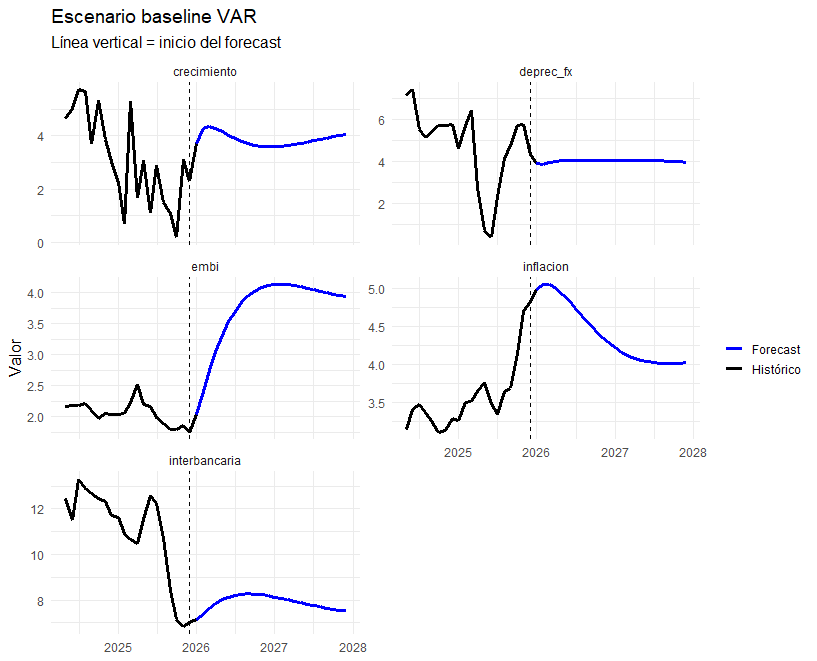
\includegraphics[width=0.6\textwidth]{escenario_base_VAR.png}
\end{figure}
\end{frame}

%------------------------------------------------
\begin{frame}{Paquete \texttt{macropenstress}: toolkit R del curso}

\textbf{Objetivo:} implementar ejercicios reproducibles de stress testing macro-financiero para sistemas de pensiones.

\vspace{0.3cm}

\begin{block}{Componentes principales}
\begin{itemize}
  \item \texttt{cargar\_datos\_pensiones()}: carga dos bases:
  \begin{itemize}
    \item \texttt{macro\_raw}: datos originales.
    \item \texttt{macro}: variables transformadas para modelación.
  \end{itemize}

  \item \texttt{escenario\_arima\_shock()}: genera baseline y escenario adverso univariado con perfil de shock $k_h$.

  \item \texttt{escenario\_var\_stress()}: genera escenarios VAR con:
  \begin{itemize}
    \item percentiles marginales,
    \item trayectoria conjunta extrema,
    \item escenario condicional.
  \end{itemize}

  \item \texttt{escenario\_var\_shock()}: aplica shocks calibrados y propaga sus efectos con la dinámica del VAR.
\end{itemize}
\end{block}

\end{frame}
%------------------------------------------------


%------------------------------------------------
\begin{frame}{Uso metodológico en stress testing previsional}

\begin{block}{Flujo de trabajo}
\[
\text{Datos macro}
\rightarrow
\text{ARIMA / VAR}
\rightarrow
\text{Escenarios}
\rightarrow
\text{Impacto previsional}
\]

\end{block}

\vspace{0.2cm}

\begin{columns}
\begin{column}{0.48\textwidth}
\textbf{Escenario baseline}
\begin{itemize}
  \item Proyección esperada.
  \item ARIMA: forecast del modelo.
  \item VAR: \texttt{predict(VAR)}.
\end{itemize}
\end{column}

\begin{column}{0.48\textwidth}
\textbf{Escenario adverso}
\begin{itemize}
  \item Shock $k_h$ en ARIMA.
  \item Monte Carlo VAR.
  \item Índice de severidad conjunta.
  \item Trayectorias condicionales.
\end{itemize}
\end{column}
\end{columns}

\vspace{0.3cm}

\begin{alertblock}{Interpretación regulatoria}
El paquete permite traducir narrativas macroeconómicas adversas en trayectorias cuantitativas coherentes para evaluar riesgos de inflación, tasas, crecimiento y depreciación cambiaria sobre fondos de pensiones.
\end{alertblock}

\end{frame}
%------------------------------------------------

% ============================================================
\begin{frame}{Construcción de escenario adverso con VAR}
\begin{block}{Idea}
El escenario adverso puede generarse imponiendo un shock inicial y dejando que el VAR propague efectos dinámicos.
\end{block}

\[
\bm y_{t+1}^{adv} =
\hat{\bm c} + \hat A_1 \bm y_t + \cdots + \hat A_p \bm y_{t-p+1}
+ \bm s_{t+1}
\]

donde $\bm s_{t+1}$ es el vector de choques calibrados.

\vspace{0.6em}
\begin{table}
\small
\begin{tabular}{lcc}
\toprule
Variable & Shock inicial & Narrativa \\
\midrule
PIB & $-2\sigma$ & Desaceleración real \\
Inflación & $+1\sigma$ & Presión de precios \\
Tasa & $+150$ pb & Endurecimiento monetario \\
FX & $+2\sigma$ & Depreciación \\
Spread & $+200$ pb & Riesgo soberano \\
\bottomrule
\end{tabular}
\end{table}
\end{frame}

% ============================================================
%------------------------------------------------
\begin{frame}{Ejercicio 2: escenario adverso determinístico con VAR}
\footnotesize
\textbf{Objetivo:} construir un escenario macro-financiero adverso calibrado y propagarlo con la dinámica estimada del VAR.

\vspace{0.2cm}

\begin{block}{Variables del sistema}
\[
Y_t =
\left[
EMBI_t,\,
crecimiento_t,\,
inflaci\acute{o}n_t,\,
interbancaria_t,\,
deprec\_fx_t
\right]'
\]
\end{block}

\begin{block}{Modelo estimado}
\[
Y_t = c + A_1Y_{t-1} + A_2Y_{t-2} + u_t
\]

El baseline se obtiene con:

\[
\widehat{Y}_{t+h}^{base} = forecast(VAR)
\]
\end{block}

\begin{alertblock}{Shock adverso calibrado}
\[
s =
\left[
2,\,-2,\,1,\,1.5,\,2
\right]
\]

Con \texttt{tipo = "sigma"}, cada shock se interpreta como múltiplo de la desviación estándar residual del VAR.
\end{alertblock}

\end{frame}
%------------------------------------------------


%------------------------------------------------
\begin{frame}[fragile]{Implementación en \texttt{macropenstress}}

\begin{lstlisting}[language=R,basicstyle=\ttfamily\scriptsize]
shock <- c(
  embi = 2,
  crecimiento = -2,
  inflacion = 1,
  interbancaria = 1.5,
  deprec_fx = 2
)

res_shock <- escenario_var_shock(
  modelo_var = var_estimado,
  shock = shock,
  h = 12,
  tipo = "sigma",
  fechas = macro$fecha,
  frecuencia = "mensual"
)
\end{lstlisting}

\begin{alertblock}{Interpretación}
El shock adverso se calibra en desviaciones estándar residuales
y el VAR propaga endógenamente la trayectoria futura.
\end{alertblock}

\end{frame}
%------------------------------------------------
% ============================================================
\begin{frame}{Interpretación VAR para política pública}
\begin{columns}
\column{0.48\textwidth}
\begin{block}{Ventajas}
\begin{itemize}
  \item Coherencia entre variables.
  \item Propagación dinámica.
  \item Lectura de canales.
  \item Útil para sensibilidad supervisora.
\end{itemize}
\end{block}

\column{0.48\textwidth}
\begin{block}{Riesgos}
\begin{itemize}
  \item Relaciones inestables en crisis.
  \item Identificación sensible al ordenamiento.
  \item Muestras pequeñas.
  \item Extrapolación fuera de historia.
\end{itemize}
\end{block}
\end{columns}

\vspace{0.4em}
\begin{block}{Mensaje regulatorio}
El VAR no ``descubre'' el escenario adverso. Ayuda a hacerlo consistente, trazable y replicable.
\end{block}
\end{frame}

% ============================================================
\section{6. Simulación Monte Carlo con \texttt{macropenstress}}

% ============================================================
\begin{frame}{¿Por qué un solo escenario no es suficiente?}
\begin{block}{Problema}
Un escenario central oculta la distribución del riesgo. Dos trayectorias pueden tener el mismo promedio, pero riesgos de cola muy distintos.
\end{block}

\begin{itemize}
  \item El baseline VAR se obtiene con \texttt{predict(VAR)}.
  \item Monte Carlo genera trayectorias alternativas usando la matriz var-cov de residuos del VAR.
  \item Los percentiles permiten construir escenarios marginales.
  \item El índice de severidad permite seleccionar trayectorias conjuntas extremas.
\end{itemize}

\vspace{0.3cm}
\begin{exampleblock}{Idea central}
Pasamos de una trayectoria esperada a una distribución de trayectorias macro-financieras.
\end{exampleblock}
\end{frame}

% ============================================================
\begin{frame}{Modelo / Herramienta: Monte Carlo sobre VAR}
Para un VAR estimado:

\[
\bm y_t =
\hat{\bm c}
+
\hat A_1 \bm y_{t-1}
+
\cdots
+
\hat A_p \bm y_{t-p}
+
\bm u_t
\]

Las innovaciones simuladas se generan como:

\[
\bm u_t^{(m)} \sim \mathcal{N}(0,\hat\Sigma_u)
\]

donde \(\hat\Sigma_u\) es la matriz var-cov de residuos del VAR.

\begin{block}{Implementación en el paquete}
\[
\texttt{escenario\_var\_stress()}
\]
permite generar baseline, percentiles marginales, trayectorias conjuntas extremas y escenarios condicionales.
\end{block}
\end{frame}

% ============================================================
\begin{frame}[fragile]{Implementación: VAR Monte Carlo con el paquete}
\begin{lstlisting}[language=R,basicstyle=\ttfamily\scriptsize]
datos <- cargar_datos_pensiones()
macro <- datos$macro

Y <- macro[, c(
  "crecimiento",
  "inflacion",
  "interbancaria",
  "deprec_fx"
)]

Y <- na.omit(Y)

var_estimado <- VAR(Y, p = 2, type = "const")

res_var <- escenario_var_stress(
  modelo_var = var_estimado,
  h = 12,
  M = 5000,
  enfoques = c("marginal"),
  percentiles = c(0.05, 0.50, 0.95),
  fechas = macro$fecha,
  frecuencia = "mensual"
)

res_var$graficos$panel
\end{lstlisting}
\end{frame}

% ============================================================
\begin{frame}[fragile]{Trayectoria conjunta extrema: índice de severidad}
\begin{lstlisting}[language=R,basicstyle=\ttfamily\scriptsize]
sim <- res_var$simulaciones

inflacion_h <- rowMeans(t(sim[, "inflacion", ]))
crecimiento_h <- rowMeans(t(sim[, "crecimiento", ]))
tasa_h <- rowMeans(t(sim[, "interbancaria", ]))
fx_h <- rowMeans(t(sim[, "deprec_fx", ]))

severity_index <-
  0.30 * as.numeric(scale(inflacion_h)) +
  0.30 * as.numeric(scale(tasa_h)) +
  0.25 * as.numeric(scale(fx_h)) -
  0.15 * as.numeric(scale(crecimiento_h))

res_conjunta <- escenario_var_stress(
  modelo_var = var_estimado,
  h = 12,
  M = 5000,
  enfoques = c("conjunta"),
  severity_by_path = severity_index,
  severity_probs = c(0.99),
  conjunta_resumen = "media",
  fechas = macro$fecha,
  frecuencia = "mensual"
)
\end{lstlisting}
\end{frame}

% ============================================================
\begin{frame}{Escenario condicional VAR}

\begin{block}{Idea}
El usuario impone una trayectoria parcial o completa para una o más variables, y el VAR genera una trayectoria coherente para el resto del sistema.
\end{block}

\[
Y_t =
\left[
crecimiento_t,\,
inflaci\acute{o}n_t,\,
interbancaria_t,\,
deprec\_fx_t
\right]'
\]

\begin{exampleblock}{Ejemplo de narrativa}
``La inflación permanece elevada durante los primeros tres meses; luego el modelo proyecta la convergencia endógena.''
\end{exampleblock}

\begin{alertblock}{Uso regulatorio}
Permite transformar una narrativa supervisora en una trayectoria macro-financiera cuantitativa.
\end{alertblock}

\end{frame}

% ============================================================
\begin{frame}[fragile]{Implementación: VAR condicional con \texttt{macropenstress}}

\begin{lstlisting}[language=R,basicstyle=\ttfamily\scriptsize]
condicion <- data.frame(
  inflacion = c(8.0, 7.5, 7.0)
)

res_condicional <- escenario_var_stress(
  modelo_var = var_estimado,
  h = 12,
  M = 5000,
  enfoques = c("condicional"),
  conditional_paths = list(
    inflacion_alta = condicion
  ),
  fill_method = "recursive",
  fechas = macro$fecha,
  frecuencia = "mensual"
)

res_condicional$graficos$panel
\end{lstlisting}

\begin{block}{Nota}
Si la trayectoria condicionada tiene menos períodos que el horizonte, el paquete completa los faltantes usando la dinámica recursiva del VAR.
\end{block}

\end{frame}

% ============================================================
\begin{frame}{Cómo convertir simulaciones en escenarios}
\begin{table}
\small
\begin{tabular}{lll}
\toprule
Escenario & Regla cuantitativa & Función \\
\midrule
Baseline & \texttt{predict(VAR)} & \texttt{escenario\_var\_stress()} \\
Marginal & Percentiles por variable & \texttt{enfoques = "marginal"} \\
Conjunto extremo & Índice de severidad & \texttt{enfoques = "conjunta"} \\
Condicional & Trayectoria impuesta & \texttt{enfoques = "condicional"} \\
Shock calibrado & Vector de shock & \texttt{escenario\_var\_shock()} \\
\bottomrule
\end{tabular}
\end{table}

\begin{block}{Cuidado}
Los percentiles marginales no siempre forman una trayectoria económicamente coherente. Para reporte regulatorio, conviene complementar con trayectoria conjunta extrema o shock calibrado.
\end{block}
\end{frame}


% ============================================================
\section{8. Taller práctico en R}

% ============================================================
% ============================================================
\begin{frame}{Escenario adverso macro-financiero}
\footnotesize
\begin{block}{Objetivo del ejercicio}
Construir un escenario de estrés a 12 meses que represente un deterioro simultáneo de las condiciones macroeconómicas y financieras, utilizando un modelo VAR como mecanismo de propagación dinámica.
\end{block}


\begin{columns}[T]

% ------------------------------------------------------------
\begin{column}{0.56\textwidth}
\footnotesize
\textbf{Narrativa económica}

\small

\begin{itemize}
  \footnotesize
    \item Aumento de la percepción de riesgo país.
    
    \item Presiones sobre el tipo de cambio y mayor inflación.
    
    \item Endurecimiento de las condiciones monetarias.
    
    \item Menor crecimiento económico producto del deterioro financiero.
    
    \item Propagación dinámica de shocks mediante el VAR.
\end{itemize}

\textbf{Variables consideradas}

\begin{itemize}
  \footnotesize
    \item Crecimiento económico
    \item Inflación
    \item Tasa interbancaria
    \item Depreciación cambiaria y EMBI
\end{itemize}

\end{column}

% ------------------------------------------------------------
\begin{column}{0.42\textwidth}
\footnotesize
\begin{block}{Choque inicial calibrado}
\small

\begin{table}
\footnotesize
\centering
\begin{tabular}{lr}
\toprule
Variable & Shock \\
\midrule
Crecimiento & -2.0 \\
Inflación & +3.0 \\
Interbancaria & +2.0 \\
Depreciación FX & +5.0 \\
EMBI & +250 \\
\bottomrule
\end{tabular}
\end{table}

\end{block}

\footnotesize
\begin{alertblock}{Resultado esperado}
Trayectorias macro-financieras coherentes y reproducibles para alimentar ejercicios de stress testing previsional.
\end{alertblock}

\end{column}

\end{columns}

\end{frame}
% ============================================================
\begin{frame}{Estructura del script del taller}
\begin{enumerate}
  \item Limpieza de sesión: \texttt{rm()}, \texttt{graphics.off()}, \texttt{detach()}.
  \item Carga del paquete: \texttt{library(macropenstress)}.
  \item Datos: \texttt{cargar\_datos\_pensiones()}.
  \item Estimación VAR: \texttt{VAR(Y, p = 2, type = "const")}.
  \item Escenario marginal: \texttt{escenario\_var\_stress()}.
  \item Trayectoria conjunta extrema: \texttt{severity\_by\_path}.
  \item Shock calibrado: \texttt{escenario\_var\_shock()}.
  \item Exportación de resultados y gráficos.
\end{enumerate}

\vspace{0.4em}
\begin{block}{Buenas prácticas}
Semilla fija, fechas explícitas, unidades claras, versiones de paquetes y separación de supuestos vs resultados.
\end{block}
\end{frame}

% ============================================================
\begin{frame}[fragile]{Implementación: objeto final de escenarios}
\begin{lstlisting}[language=R,basicstyle=\ttfamily\scriptsize]
escenarios <- bind_rows(
  res_var$resultados %>%
    mutate(fuente = "VAR Monte Carlo"),
  res_conjunta$resultados %>%
    mutate(fuente = "Severidad conjunta"),
  res_shock$resultados %>%
    mutate(fuente = "Shock calibrado")
) %>%
  mutate(
    modulo_origen = "M3",
    fecha_generacion = Sys.Date()
  )

write.csv(
  escenarios,
  "escenarios_macrofinancieros.csv",
  row.names = FALSE
)
\end{lstlisting}
\end{frame}

% ============================================================
\begin{frame}{Guía de trabajo en grupos}
\begin{table}
\small
\begin{tabular}{p{2.7cm}p{4.2cm}p{4.2cm}}
\toprule
Grupo & Foco técnico & Pregunta de decisión \\
\midrule
A & VAR baseline & ¿El forecast es razonable? \\
B & Monte Carlo marginal & ¿Qué percentil usar como alerta? \\
C & Severidad conjunta & ¿Qué trayectoria representa crisis sistémica? \\
D & Shock calibrado & ¿La narrativa adversa es plausible? \\
\bottomrule
\end{tabular}
\end{table}

\begin{block}{Discusión plenaria}
Cada grupo debe explicar la logica de su escenario.
\end{block}
\end{frame}

% ============================================================
\section{Taller práctico: VAR para economía abierta}

% ============================================================
\begin{frame}{Taller práctico: economía abierta}

\begin{block}{Objetivo}
Construir escenarios macro-financieros para una economía pequeña y abierta utilizando un modelo VAR que incorpore variables domésticas y externas.
\end{block}

\begin{itemize}
    \item Evaluar la transmisión de shocks externos hacia la economía local.
    \item Simular trayectorias para alimentar ejercicios de stress testing.
    \item Comparar escenarios baseline, adverso externo, conjunto extremo y condicional.
\end{itemize}

\end{frame}

% ============================================================
\begin{frame}{Variables del modelo VAR}

\begin{columns}[T]

\begin{column}{0.48\textwidth}
\begin{block}{Variables domésticas}
\small
\begin{itemize}
    \item Crecimiento económico
    \item Inflación
    \item Tasa interbancaria
    \item Depreciación cambiaria
    \item EMBI
\end{itemize}
\end{block}
\end{column}

\begin{column}{0.48\textwidth}
\begin{block}{Variables externas}
\small
\begin{itemize}
    \item Precio internacional del petróleo
    \item Tasa de interés de la FED
    \item Crecimiento económico de EE.UU.
\end{itemize}
\end{block}
\end{column}

\end{columns}

\vspace{0.5em}

\begin{alertblock}{Idea central}
El modelo permite estudiar cómo un deterioro del entorno internacional se transmite a inflación, tipo de cambio, tasas, crecimiento y riesgo país.
\end{alertblock}

\end{frame}

% ============================================================
\begin{frame}{Narrativa del escenario adverso externo}

\begin{block}{Escenario}
A partir del inicio del horizonte de proyección, la economía enfrenta un deterioro del entorno internacional.
\end{block}

\begin{itemize}
    \item Aumento del precio internacional del petróleo.
    \item Incremento de la tasa de interés de la FED.
    \item Desaceleración del crecimiento de EE.UU.
    \item Presiones sobre el tipo de cambio.
    \item Aumento del EMBI.
    \item Mayor inflación y respuesta de la tasa doméstica.
    \item Menor crecimiento económico.
\end{itemize}

\end{frame}

% ============================================================
\begin{frame}{Calibración del shock adverso externo}

\begin{block}{Unidades}
Los shocks están expresados como múltiplos de la desviación estándar histórica de cada variable.
\end{block}

\begin{table}
\centering
\small
\begin{tabular}{lcc}
\toprule
Variable & Shock & Interpretación \\
\midrule
Crecimiento & $-1.5$ & menor actividad \\
Inflación & $+1.5$ & mayor presión inflacionaria \\
Interbancaria & $+1.0$ & respuesta monetaria \\
Depreciación FX & $+2.0$ & presión cambiaria \\
EMBI & $+2.0$ & mayor riesgo país \\
Precio petróleo & $+2.5$ & shock externo de costos \\
Tasa FED & $+2.0$ & condiciones financieras externas \\
Crecimiento EE.UU. & $-2.0$ & menor demanda externa \\
\bottomrule
\end{tabular}
\end{table}

\end{frame}

% ============================================================
\begin{frame}[fragile]{Estructura del script}

\small

\begin{verbatim}
# 1. Limpieza de sesión
# 2. Carga de paquetes
# 3. Parámetros generales
# 4. Carga y preparación de datos
# 5. Estimación del VAR
# 6. Escenario adverso externo
# 7. Escenario conjunto extremo
# 8. Escenario condicional
# 9. Tablas y gráficos
\end{verbatim}

\begin{block}{Producto final}
Un script reproducible en R que genere escenarios macro-financieros de economía abierta.
\end{block}

\end{frame}

% ============================================================
\begin{frame}[fragile]{Código base: variables del VAR}

\small

\begin{verbatim}
variables_var <- c(
  "crecimiento",
  "inflacion",
  "interbancaria",
  "deprec_fx",
  "embi",
  "oil_price",
  "fed_rate",
  "us_growth"
)
\end{verbatim}

\begin{alertblock}{Nota}
Las tres últimas variables representan el bloque externo del modelo.
\end{alertblock}

\end{frame}

% ============================================================
\begin{frame}[fragile]{Código base: estimación del VAR}

\small

\begin{verbatim}
Y <- macro %>%
  select(all_of(variables_var)) %>%
  na.omit()

modelo_var <- VAR(
  y = Y,
  p = 2,
  type = "const"
)

roots(modelo_var)
\end{verbatim}

\begin{block}{Diagnóstico}
Las raíces del VAR deben estar dentro del círculo unitario para que el modelo sea estable.
\end{block}

\end{frame}

% ============================================================
\begin{frame}[fragile]{Código base: shock adverso externo}

\small

\begin{verbatim}
shock_externo <- c(
  crecimiento   = -1.5,
  inflacion     =  1.5,
  interbancaria =  1.0,
  deprec_fx     =  2.0,
  embi          =  2.0,
  oil_price     =  2.5,
  fed_rate      =  2.0,
  us_growth     = -2.0
)

adverso_externo <- escenario_var_shock(
  modelo_var = modelo_var,
  h = h,
  shock = shock_externo
)
\end{verbatim}

\end{frame}

% ============================================================
\begin{frame}{Índice de severidad conjunta}

\begin{block}{Idea}
El escenario conjunto extremo no se obtiene tomando percentiles variable por variable.
\end{block}

\begin{enumerate}
    \item Se simulan muchas trayectorias conjuntas del VAR.
    \item Se calcula un índice de severidad para cada trayectoria.
    \item Se selecciona la trayectoria ubicada en la cola adversa.
\end{enumerate}

\vspace{0.5em}

\begin{alertblock}{Variables que aumentan la severidad}
Mayor inflación, tasa interbancaria, depreciación, EMBI, precio del petróleo y tasa FED; menor crecimiento local y menor crecimiento de EE.UU.
\end{alertblock}

\end{frame}

% ============================================================
\begin{frame}[fragile]{Código base: escenario condicional}

\small

\begin{verbatim}
restricciones <- tibble(
  crecimiento = c(1.0, 1.2, 1.5, 1.8, 2.0, rep(2.5, h - 5)),
  inflacion = c(8.0, 7.5, 7.0, 6.5, 6.0, rep(5.5, h - 5)),
  interbancaria = c(9.0, 9.0, 8.75, 8.5, 8.25, rep(8.0, h - 5)),
  deprec_fx = c(8.0, 7.0, 6.0, 5.0, 4.5, rep(4.0, h - 5)),
  embi = c(650, 625, 600, 575, 550, rep(525, h - 5)),
  oil_price = c(95, 92, 90, 88, 85, rep(82, h - 5)),
  fed_rate = c(6.0, 5.8, 5.5, 5.25, 5.0, rep(4.75, h - 5)),
  us_growth = c(0.5, 0.8, 1.0, 1.2, 1.5, rep(1.8, h - 5))
)
\end{verbatim}

\end{frame}

% ============================================================
\begin{frame}{Entregable del ejercicio}

\begin{block}{Producto final}
Una tabla consolidada con cinco períodos históricos y las trayectorias proyectadas para cada escenario.
\end{block}

\begin{table}
\centering
\small
\begin{tabular}{llll}
\toprule
Periodo & Escenario & Variable & Valor \\
\midrule
2025-08 & Histórico & Inflación & 4.2 \\
2025-09 & Histórico & Inflación & 4.5 \\
2026-01 & Baseline & Inflación & 4.8 \\
2026-01 & Adverso externo & Inflación & 7.5 \\
2026-01 & Condicional & Inflación & 8.0 \\
\bottomrule
\end{tabular}
\end{table}

\end{frame}

% ============================================================
\begin{frame}{Preguntas guía para los grupos}

\begin{enumerate}
    \item ¿Cuál es el shock externo dominante en el escenario?
    \item ¿Qué variable doméstica reacciona con mayor intensidad?
    \item ¿Cómo se transmite el shock del petróleo a la inflación?
    \item ¿Qué rol juega la tasa FED en el EMBI y el tipo de cambio?
    \item ¿Qué escenario luce más severo para el portafolio previsional?
\end{enumerate}

\end{frame}

% ============================================================
\end{document}
